% !TEX encoding = UTF-8 Unicode
% !TEX TS-program = pdflatex

 \documentclass[%
    corpo=11pt,
    twoside,
    %stile=classica,
    oldstyle,
    tipotesi=magistrale,
    %evenboxes,
]{toptesi}

\usepackage[utf8]{inputenc}		% codifica d'entrata
\usepackage[T1]{fontenc}		% codifica dei font
\usepackage{pdfx}				% to save metadata for long term storage of the pdf file.
\usepackage[backend=biber]{biblatex}
\usepackage{mathpazo}			% font
\usepackage[scaled]{beramono}	% monospace font
\usepackage{hyperref}			% for links
\usepackage{xcolor}				% for colors
\usepackage{longtable,array,booktabs,tabularx}	% for tables
\usepackage{siunitx}			% for measurement units
\usepackage{minted}

\usepackage{lipsum}

% Input settings file
\hypersetup{
	pdfpagemode={UseOutlines},
	bookmarksopen,
	pdfstartview={FitH},
	colorlinks,
	linkcolor={blue},
	citecolor={blue},
	urlcolor={blue}
}

\usemintedstyle{algol_nu}

\definecolor{codebackground}{RGB}{0.95, 0.95, 0.95}

\newmintedfile[bashcode]{bash}{
	bgcolor=code_background,
	fontfamily=tt,
	linenos=true,
	numberblanklines=true,
	numbersep=5pt,
	gobble=0,
	frame=leftline,
	framerule=0.4pt,
	framesep=2mm,
	funcnamehighlighting=true,
	tabsize=4,
	obeytabs=false,
	mathescape=false
	samepage=false, % with this setting you can force the list to appear on the same page
	showspaces=false,
	showtabs =false,
	texcl=false,
}


% Load bibliography databases
\addbibresource{thesis_bibliography.bib}

% Construct the indexes
\makeindex


\begin{document}\errorcontextlines=9
	
	\begin{frontespizio}

	\ateneo{Università degli Studi di Brescia}
	
	\titolo{Titolooooo}
	\sottotitolo{Metodo dei satelliti medicei}
	
	\corsodilaurea{Ingegneria dell'Automazione Industriale}
	\candidato{Alghisi Giovanni}[719738]
	
	\relatore{Prof.\ Francesco Gringoli}
	
	\sedutadilaurea{\textsc{Anno~accademico} 2022-2023}
	
	\logosede{Front/thesis_unibs_logo.pdf}

\end{frontespizio}

	
	% Switch to english
	\english
	
	\tableofcontents

	% !TEX root = ../toptesi-scudo-example.tex
% !TEX encoding = UTF-8 Unicode
%***********************************************************************
%*********************************** First Chapter 
%***********************************************************************

\chapter{First Chapter Title}  %Title of the First Chapter
\label{chapter 1}
    \graphicspath{{Chapter1/Images/}}
    
    \begin{minted}{bash}
#!/bin/bash
echo "Hello, World!"

for file in *; do
    vim $file
    echo "Bellissimoooo $0, $1"
done
    \end{minted}


%**************************** %First Section  ****************************
\section[Introduction to PhD thesis template]{Introduction to PhD thesis template\footnote{The greatest part of this example file was written by an unknown past ScuDo student who did not sign his/her work; s/he just put the file in Internet, and apparently the other ScuDo students highly appreciated this thesis template. As the author of the TOPtesi bundle, with approval of the ScuDo Director, I included this example into the bundle. With the first public release, the only modification I made was to use the fake logo image in order to protect the Doctoral School copyright; then I added a few modifications in order to upgrade certain links and some procedures, since the TOPtesi bundle has been upgraded after the first public release of this file.}} %Section - 1.1 
\label{section 1.1} % here you can label the section to refer it inside the text

Welcome to this \LaTeX\ Thesis Template for writing your PhD thesis using the \LaTeX{} typesetting system. If you are writing a thesis (or will be in the future) and its subject is technical or mathematical (though it doesn't have to be), then creating it in \LaTeX\ is highly recommended.

\LaTeX\ is a mark up language and its associated typesetting programs such as pdfLaTeX, LuaLaTeX, or XeLaTeX professionally typeset documents of any length,  that run to hundreds or thousands of pages long. With simple mark-up commands, it automatically sets out the table of contents, margins, page headers and footers and keeps the formatting consistent and beautiful. One of its main strengths is the way it can easily typeset mathematics, even advanced mathematics. Even if those equations are the most horribly twisted and most difficult mathematical problems that can only be solved on a super-computer, you can at least count on \LaTeX\ to make them look stunning: \cite{lamport1994latex, misc:Lshort}. Please see appendix~\ref{Appendix1} for the instruction on how to install a complete \TeX\ system.

Along with this document you have access to its \LaTeX\ source file (\textbf{toptesi-scudo-example.tex}) including different partitions. Inside each part there are instructive comments explaining the options for different commands. The default commands are designed and recommended by PhD school of Politecnico di Torino. In this tutorial the  essential commands to write a scientific document are listed and briefly explained.  




%************************ Second Section  ***********************
\section{Getting started with this template}  %Section - 1.2 
\label{section1.2}
If you are familiar with \LaTeX, then you should explore the directory structure of the template and then proceed to place your own information into a configuration file with extension \texttt{.cfg} and a name that matches exactly your main file name; pay attention to upper and lower case letters. You can then modify the rest of this file to your unique specifications based on your course. Chapter \ref{chapter 2} will help you do this.

If you are new to \LaTeX\ it is recommended that you carry on reading through the rest of the information in this document. The style of this template is confirmed and recommended by the Doctoral School of Politecnico di Torino (ScuDo).

%************************* Third Section  ***************************
\section{What is included in this template}
\label{section 1.3}

\subsection{Folders}

This template comes as a single zip file that expands out to several files and folders. The folder names are mostly self-explanatory:

\textbf{Chapters}: these are the folders where you put the thesis chapters.  Each chapter should go in its own separate \textbf{.tex} file and folder. Each chapter folder might contains a \textbf{Figs} subfolder which contains all figures for the chapter. A thesis usually has about five to six chapters, though there is no strict rule on this. For example they can be split as:
\begin{itemize}
	\item Chapter 1: Introduction to the thesis topic
	\item Chapter 2: Background information and theory
	\item Chapter 3: (Laboratory) experimental setup
	\item Chapter 4: Details of experiments
	\item Chapter 5: Discussion of the experimental results
	\item Chapter 6: Conclusion and future directions
\end{itemize}
This chapter layout is specialised for the experimental sciences.

\textbf{Appendices}: these are the folders where you put the appendices. Each appendix should go into its own appendix folder with its \textbf{.tex} file and figures; should the figures be in large numbers, a subordinate folder to hold all the figure files might be created.

\subsection{Files}

Included are also several files, most of them are plain text and you can see their contents in a text editor. After initial compilation, you will see that more auxiliary files are created by the typesetting and \texttt{biber} programs; you don't need to delete them or worry about:

\noindent\textbf{toptesi-scudo-example.pdf}: this is your beautifully typeset thesis (in PDF file format) created by the typesetting program you chose to use. It is already supplied with the source files and after you compile the example you should get an identical version.

\noindent\textbf{toptesi-scudo-example.tex}: this is an important file. This is the file that you should move to your working folder and, after changing its name, you may use it as a template to create your own thesis; you compile it to produce a PDF file. It contains the framework and constructs that tell \LaTeX\ how to layout the thesis. It is heavily commented so you can read exactly what each line of code does and why it is there. 
 For your thesis you have to duplicate the example files with a different name, and you substitute their contents by writing your thesis following the same scheme.

Files that are \emph{not} included, but are created by \LaTeX\ as auxiliary files include:\textbf{.aux}, \textbf{.bbl}, \textbf{.blg}, \textbf{.lof}, \textbf{.log}, \textbf{.lot} and \textbf{.out} files: they are auxiliary files generated by \LaTeX; if they are deleted \LaTeX\ simply regenerates them when you run the main \textbf{.tex} file again. But since they contains useful information for the typesetting program, it is better that you eventually delete them only when the thesis is finished, printed, and defended. 

%********************** Forth Section  ****************************

\section{Filling in your information in the thesis main and subsidiary files}
\label{section 1.4}

You need to personalise the thesis template and make it your own by filling in your own information. This is done by editing the main renamed \textbf{.tex} file with your favorite \LaTeX\ friendly editor (See Appendix~\ref{Appendix1}).

Open the file and scroll down to the second large block titled \emph{ThesisTitlePage} where you can see the entries for \emph{Author}, \emph{Supervisors}, etc. Fill out the information about your thesis, yourself and your school. When you have done this, save the file and recompile your main file. All the information you filled-in should now be in the PDF, complete with web links. You can now begin your thesis proper!
Remember that sooner or later you have to come back to the first block, in order to adjust the metadata to your particular thesis.

The \textbf{toptesi-scudo-example.tex} file contains the structure of the thesis. There are plenty of written comments that explain what pages, sections and formatting the \LaTeX\ code is creating. 

Begin by checking that your information on the title page is correct. The next page contains a one line (or more) dedication; you may write a dedication, but in Europe this habit is not so frequent. Next come the acknowledgements. On this page acknowledge the people that gave you some support during the development of the research you made for your doctorate program. Do not acknowledge the members of your family nor the professors who supervised and advised you during your research; they did so as their duty as members of the institutions where you followed your doctorate program. Following this section  there is the abstract/summary page which describes  your work in a condensed way; it can almost be used as a standalone document to describe what you have done. 

The contents pages, list of figures and tables are all taken care of for you and you do not need to manually create or edit.  Finally, there is the block where the chapters are included. Uncomment the lines (delete the \% character) as you write the chapters. Each chapter should be written in its own file and possibly put into its own chapter sub-folder. Similarly for the appendices, uncomment the lines as you need them. Each appendix should go into its own file and possibly placed in its own appendix sub-folder.

After the preamble, chapters and appendices, eventually the program inserts the bibliography, possibly a nomenclature list, an index, or other similar information. The bibliography \textbf{numbered} style is used for the bibliography and is a fully featured style that will even include links to where the referenced paper can be found online; it satisfies the standard of the IEEE Transactions in the fields of interest of this Institution and it is assumed to be the style used in the PhD theses concerning these fields; of course in other scientific domains other styles may be used; see below how the default style may be overridden. 
In any case do not underestimate how grateful your reader will be to find that a reference to a paper is just a click away. Of course, this relies on you putting the URL information into the \textbf{.bib} file. Unfortunately URLs are sort of volatile; prefer references to printed material, that can be found in (almost) any library, or links to reliable web archives. For URLs, remember to specify the date when you last visited the web site; it is useful for the reader, but is also compulsory according to some ISO regulations.

Notice that the facilities necessary to produce one or more bibliographies with the numbered style are already provided by the \texttt{toptesi-scudo} option to the \texttt{toptesi} class. But even if these facilities are  hardwired into the class and its subsidiary files, it is possible to bypass them. 

If you prefer a different style, you can do it the way we did it in typesetting this example document. You simply have to specify the special option \texttt{mybibliostyle} among the other class options; then you have to add to your document preamble the necessary code to include the packages you prefer, and to specify the name of the bibliographic database(s) \texttt{.bib}. You do not need to enclose this code into a conditional statement as it has been done in this example; but of course it is not forbidden.

Here we specified the above option and we used the conditional statement to enclose another set of packages and settings. Try recompiling the source file of this document without editing it, and run the usual processing task  sequence: lualatex, biber, lualatex, lualatex; then examine the typeset bibliography; it will use the \textbf{author-year} style.
Then comment out the line containing the \texttt{mybibliostyle} option and repeat the usual processing tasks: lualatex, biber, lualatex, lualatex. And there you are with the default \textbf{numbered} style, as described above.

In order to change style the bundle TOPtesi does not require programming acrobatics; but before changing style inquire with your PhD supervisor or with the School Director if your preferred bibliography style may be accepted by the School. Remember, though, that if your thesis deals with the IEEE Transactions disciplines, you should use the default settings and you should refrain from using the \texttt{mybibliostyle} option.

Please, take notice that the \texttt{toptesi-scudo-example.bib} file is just an example that contains some entries just to show how bibliography databases are formed and how bibliographies are typeset. The records in this file are not necessarily complete, in the sense that some of them do not contain the full and correct necessary and supplementary information required by the regulation \textsc{iso 626}. It's up to you to enter the full and correct information in your own \texttt{.bib} file.




	
	%% !TEX root = ../toptesi-scudo-example.tex
% !TEX encoding = UTF-8 Unicode
%**********************************************************************%****************************** Second Chapter %**********************************************************************
\chapter{Second Chapter Title}
\label{chapter 2}
    \graphicspath{{Chapter2/}}
    
%****************************** First Section ****************
\section{Basic text and referring hints}
%*************************************************************

\LaTeX\ gives the possibility to bold a \textbf{word}, or a \textbf{phrase containing several words}, or mathematical equations like $\mathbf{A=B+C}$. \textit{Italic}\footnote{ Never \underline{underline} any part of your text to emphasise it: it is bad typography! Underlining was used in the old times of mechanical typewriter when there was no other means to emphasise text.} commands are designed to be used to emphasise some text. Text sizing requires other optional commands:
{\small Word}, {\large Word}, {\Large Word}.

The various size commands are the following:
 \texttt{\string\Huge}.
 \texttt{\string\huge}.
 \texttt{\string\LARGE}.
 \texttt{\string\Large}.
 \texttt{\string\large}.
 \texttt{\string\normalsize} (default),
 \texttt{\string\small}.
 \texttt{\string\footnotesize}.
 \texttt{\string\scriptsize}.
 \texttt{\string\tiny}.

{\tolerance = 3000 Referring to sections, chapters, equations and \dots, is possible by means of the \verb|\ref{label}| command. It is necessary to insert \verb|\label{section label}| for each desired section, and chapter, and \dots, then making a reference to them in any part of the text. For example in chapter~\ref{chapter 1} we introduced the template and in section~\ref{section 1.3} different folders and template files were described. Figure~\ref{fig:Greek} shows the Greek letter codes in \LaTeX.\par}

In \LaTeX\footnote{Here there is the footnote explanation about the word \LaTeX} it is possible to typeset footnote explanations. 

You can also insert web links, if you do, make sure you use the full URL, including the \{http://\} part in the URL. As an example, by using the code: 
\begin{verbatim}
\href{http://www.polito.it}{polito website} 
\end{verbatim} 
you get \href{http://www.polito.it}{polito website}. If you don't want to link the URL to a name, remove the name and just write  \verb|\url{http://www.polito.it}|. This is the result: (\url{http://www.polito.it}).

When quoting some  phrases pay attention to use the proper quotation marks “\dots” (that are not accessible from normal keyboards unless you use a specific \emph{Charater table}), of your editor, or special editor shortcuts, or the standard \TeX\ ligature \verb|``\dots''|, that produces~``\dots''.

%************************************* 
% Second Section  
\section{Writing mathematical equations in \LaTeX} %Section - 2.2
\label{section 2.2}
%*************************************

% Uncomment this line, if you have siunitx package loaded.
%The SI Units for dynamic viscosity is \si{\newton\second\per\metre\squared}.
As an in-line equation example we can refer the most famous equation in the world: $E^2 = (m_0c^2)^2 + (pc)^2$, which is known as the \textbf{energy-mass-momentum} relation. You can write an equation in an \textbf{equation} environment of \LaTeX, for example “Cauchy's Integral Formula” which is automatically given an equation number (tag) by \LaTeX\ like this\footnote{% 
% In footnotes the \verb command is fragile (LaTeX fault; when using
% package fancyvrb this limitation disappears).
% The strange construct "\texttt{\string...}" is a way to bypass the \verb
% fragility
Here $\iota$ is used in place of an upright `i' or `j', just to show an example, and to have another item of math Greek to list in the nomenclature typeset at the end of the example. An upright `i' or `j' is required when the \textsc{iso} regulations concerning math for “physics and technology" must be fulfilled. the TOPtesi module \texttt{toptesi-scudo} provides the commands \texttt{\string\iu} and its alias \texttt{\string\gei} to set the “imaginary unit”  with `j', as is commonly done in the IEEE Transactions; if you want to use `i', redefine \texttt{\string\iu}, but leave alone \texttt{\string\gei} so as to retain its meaning. \textbf{Never ever use the math Greek \string\iota\ in place of the imaginary unit.}}:
\begin{verbatim}
\begin{equation}
CIF\colon \qquad F_0^j(a) =\frac{1}{2\pi \iota} 
    \oint_{\gamma} \frac{F_0^j(z)}{z - a} \diff z
\end{equation}
\end{verbatim}
This will produce “Cauchy's Integral Formula” equation:
\begin{equation}
CIF\colon \qquad F_0^j(a) = \frac{1}{2\pi \iota} 
    \oint_{\gamma} \frac{F_0^j(z)}{z - a} \diff z
\label{equ:Cauchy}
\end{equation}

In equation\eqref{equ:Cauchy} notice the \verb|\diff| command needed to fulfil the ISO recommendations on math writing in science and technology. The spacing before and after the symbol is correct; it accepts also exponents as for example in:
\begin{equation}
\frac{\diff^2 x}{\diff t^2} + \frac{\diff x}{\diff t} + c x= f(t)
\end{equation}


As you see the equation is tagged automatically according to the chapter. It is also possible to personalise the equation tag:
\begin{equation}
\centering
\tag{Cauchy integral formula}
F_0^j(a) = \frac{1}{2\pi \iota} \oint_{\gamma} \frac{F_0^j(z)}{z - a} \diff z
\end{equation}
with the following code:
\begin{verbatim}
\begin{equation}
\centering
\tag{Cauchy integral formula}
F_0^j(a) = \frac{1}{2\pi \iota} 
    \oint_{\gamma} \frac{F_0^j(z)}{z - a} \diff z
\end{equation}
\end{verbatim}
Notice, though, that tagging with long phrases leaves less space on the line, and the formula is centred within this remaining space.


If there are several equations that you need to align vertically, the \textbf{align} environment will do it:
\begin{align*}
	x&=5y          &  w &=-z             &  a&=b-c\\
	2x&=-y         &  3w&=\frac{1}{2}z   &  a&=3b \\
	-4 + 5x&=2+y   &  w+2&=-1+w          &  ab&=\frac{-1}{3}cb
\end{align*}

Math equation environments that use  the asterisk * produce unnumbered   equations.

%*********************************************
\section{How to create an index}% 3rd section
%*********************************************

The package \texttt{imakeidx}\index{package!imakeidx@\texttt{imakeidx}} loaded in the preamble is suited to create one ore more indices without any specific action by the user except the (obvious) marking of the words\index{words} or phrases\index{phrases} to list in this particular part of the thesis.

The mandatory \texttt{\string\makeindex} command in the preamble is necessary to activate the \texttt{\string\index}\index{index@\texttt{\string\index}} command; without this activation this command does not do anything. At the same time the \texttt{\string\makeindex} command accepts a list of \textit{key = value} options by which it is possible to fully configure the index features; in this sample template file only the \textsl{intoc} option has been specified, in order to have the index name and page listed in the table of contents.

Read the \texttt{imakeidx} package documentation in order to use the package at its best.

%**************************************************
\section{How to create a nomenclature}% 4th section
%**************************************************

Somewhere in the thesis you might have to configure the nomenclature list you are going to create; the necessary command is \texttt{\string\nomenclature} that requires two mandatory arguments: the first one is the ``acronym'' you want to list, and the second is its meaning. 
\nomenclature[Z]{$CIF$}{Cauchy's Integral Formula}% letter Z is for Acronyms 
\nomenclature[A]{$F$}{complex function}% letter A is for Roman symbols
\nomenclature[G]{$\pi$}{ $\simeq 3.14159\ldots$}% letter G is for Greek Symbols
\nomenclature[G]{$\iota$}{imaginary unit $\sqrt{-1}$; never use the Greek iota to denote the imaginary unit}% never actually use \iota in place of \iu                      
\nomenclature[G]{$\gamma$}{a simply closed curve on a complex plane}  
\nomenclature[X]{$\oint_\gamma$}{integration along a closed curve $\gamma$}% first letter X is for Other Symbols
\nomenclature[R]{$j$}{superscript index}% first letter R is for superscripts
\nomenclature[S]{$0$}{subscript index}% first letter S is for subscripts
%%%
%%% Letters Z, A, G, X, R, S, are just place holders for the actual
%%% labels in the nomenclature list. they were defined in the
%%% toptesi-scudo.sty fiile.

To create the \textbf{Nomenclature} you need to issue the 
\verb|\nomenclature| command for each symbol you want to have included in the nomenclature list. The best place for this command is immediately after you introduce the symbol for the first time. For  equation~\eqref{equ:Cauchy} in the previous section we set:
\bgroup\small
\begin{verbatim}
\nomenclature[Z]{$CIF$}{Cauchy's Integral Formula}
\nomenclature[A]{$F$}{complex function}
\nomenclature[G]{$\pi$}{$\simeq 3.14159\ldots$}
\nomenclature[G]{$\iota$}{unit imaginary number $\sqrt{-1}$}
\nomenclature[G]{$\gamma$}{a closed curve on a complex plane}
\nomenclature[X]{$\oint_\gamma$}{integration along a closed curve $\gamma$} 
\nomenclature[R]{$j$}{superscript index}
\nomenclature[S]{$0$}{subscript index}
% letter Z is for Acronyms, A is for Roman symbols,
% G is for Greek Symbols, X is for Other Symbols, 
% R is for superscripts, S is for subscripts
\end{verbatim}
\egroup
The above list of nomenclature entries is pretty naïve; if you decide to write a nomenclature, provide one that contains real useful information. If you follow the nomenclature information published in several texts, you do not need to write a nomenclature of physical symbols; if you need a link to a technical reference easily downloadable from the internet, try \texttt{sp811.pdf} downloadable by clicking on this active link: \url{http://www.nist.gov/customcf/get_pdf.cfm?pub_id=200349}. Apparently this document speaks about the correct usage of SI units of measure; but in practice it gives very good information on writing about measures in a technical document and contains lots of lists of symbols for indicating physical quantities. 

You do not have to do anything special to typeset the nomenclature section, except of course inserting the \texttt{\string\printnomencl} command in the back matter of your thesis before or after the section containing the bibliography, but before a possible index. The extension to TOPtesi made by  file \texttt{topesi-scudo.sty} provides to launch in background the necessary external programs with suitable options so as to exploit the \texttt{shell escape} functionality of pdfLaTeX and XeLaTeX; LuaLaTeX does not natively provide this functionality, but the above extension package provides the Lua language commands so as to execute the necessary actions as it would happen with the other typesetting engines. Should the external program find some error in the entry data, it might issue error messages in the .log file of the main file of your thesis; read he diagnostic messages and provide the necessary corrections. Matter of fact this example file is being typeset with LuaLaTeX, and the nomenclature appears regularly close to the end of the PDF file, without issuing any command-line command.

Your task, then, remains that of marking the necessary entries as shown in the preceding example paragraph.

% Several people use explicit vertical space; this is a typical beginners
% error; in any case prefer small units of measure so as to avoid decimals
% and null integer parts; do not write \vspace{0.5cm}, and prefer
% \vspace{5mm}.


%******************************************************
% Fifth Section  
\section{List formatting in \LaTeX}\label{section 2.3}
%******************************************************

Convenient and predictable list formatting is one of the many advantages of using \LaTeX. \LaTeX\ distinguishes between three different enumeration/itemisation environments: 
%
\begin{itemize}
	\item \texttt{enumerate} for an enumerated list,
	\item \texttt{itemize} for a bullet list,
	\item \texttt{description} for a descriptive list.
\end{itemize}
All lists follow a basic format and each of them provides four levels, which means you can have nested lists of up to four levels. Never set up nested lists up to level four; level 2 is OK; level 3 may be too much; level 4 corresponds to a list very difficult to read and understand. After all, lists are made up to display information in a structured way so as to make their contents easier to understand.

\subsection{Enumerate}
Never start a section with a list; try to always write some introductory text before the list. Items in an enumeration are each made up of complete sentences, that form one or more paragraphs. Every item starts with a capital letter and finishes with a full stop.
\begin{enumerate}
	\item The first topic is ``Good''.
	\item The second topic is ``Intermediate'' (Lev. 1).
	\begin{enumerate}
		\item The first subtopic is ``high intermediate'' (Lev. 2).
		\item The second subtopic is ``low intermediate''.
		\begin{enumerate}
			\item The first subsubtopic is ``very low intermediate'' (Lev. 3).
			\begin{enumerate}
				\item The first subsubsubtopic is ``too low intermediate'' (Lev. 4).
			\end{enumerate}
		\end{enumerate}
	\end{enumerate}
	\item The third topic is ``Bad.
\end{enumerate}

Sub-items in an enumeration may be bulleted lists; the opposite, enumeration list embedded into a bulleted list, is an error.

\subsection{Itemize}
A bulleted list is part of the introductory test; therefore no item starts with a capital letter, and no item but the last, ends with a full stop; other items my finish with a comma or a semicolon, but the elliptic form without final punctuation is OK in technical texts. therefore:
\begin{itemize}
	\item the first topic is ``Good''
    \item the second topic is ``Intermediate''
    \begin{itemize}
	     \item the first subtopic is ``high intermediate''
	     \item the second subtopic is ``low intermediate''
	     \begin{itemize}
		      \item the first subsubtopic is ``very low intermediate''
	     \end{itemize}
\end{itemize}
\item the third topic is ``Bad''
\end{itemize}
Some text may follow a bulleted list; it continues the sentence that contained the list if the first line is not indented and starts with a lowercase letter. If it starts with an uppercase letter, but the first line is not indented, it is a new sentence that continues the paragraph that contains the list. If this text starts with an indented line with an uppercase initial in the first word, a  new paragraph is started. On the contrary, if this text has the first line indented, but the initial is lowercase, there is an error; you left a blank line after the list source  and the first line of the following text; please correct it.

\subsection{Description}
The description environment follows the same rules of the enumeration. The real difference is that the list has words or phrases as item marks, instead of numbers. The word or phrase to be described or defined is the ``optional'' argument of command \texttt{\string\item}; the word ``optional'' is quoted, because in case of a description environment the command argument is mandatory, because it is nonsense to give the description of nothing.
\begin{description}
	\item [The first topic] is ``Good''.
    \item [The second topic] is ``Intermediate''.
    \begin{description}
	      \item [The first subtopic] is ``high intermediate''.
	      \item [The second subtopic] is ``low intermediate''.
	      \begin{description}
		        \item [The first subsubtopic] is ``very low intermediate''.
	      \end{description}
\end{description}
\item [The third topic] is ``Bad''
\end{description}

\subsection{Comments on lists}
In the previous examples the ``Good'', \dots, ``Bad'' quoted qualifiers do not express the validity of the nested level; they are just words. Notice that the quotes were not created with the ASCII straight double quote sign \verb|"| that does not distinguish open from closed quotes; open quotes were created with the \TeX\ ligature \verb|``| and closed quotes are created with the other \TeX\ ligature \verb|''|. When using LuaLaTeX or XeLaTeX, if the keyboard has facilities to enter non ASCII characters, it would be possible to enter directly \verb|“| and \verb|”|. When using an Italian keyboard it is difficult to enter the ligature \verb|``|; with such a keyboard you need to ask your shell editor to enter a special symbol, by means of something called ``Character Table'' or ``Symbol Table''.

%********************************** 
% Sixth Section  
\section{Figures}\label{section 2.4}
%**********************************

Hopefully there will be many figures in your thesis (that should be placed in the \textbf{Figs} sub-folder in each chapter folder). The way to insert figures into your thesis is to use a code template like this:
\begin{verbatim}
\begin{figure}[tbp] 
\centering    
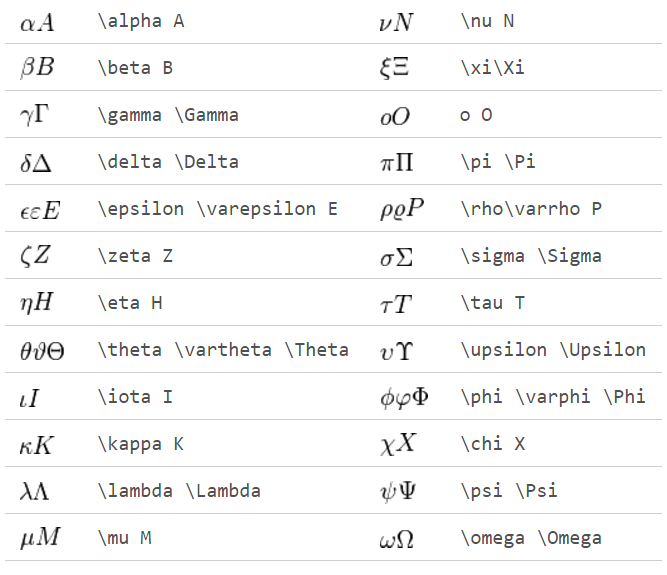
\includegraphics[width=1.0\textwidth]{Greek_letters}
\caption[Greek letters in \LaTeX]%
      {List of math greek letters in \LaTeX}
\label{fig:Greek}
\end{figure}
\end{verbatim}
Also look in the source file. Putting this code into the source file produces the Figure~\ref{fig:Greek} that you can see in the figure below. By changing the value of figure width (\texttt{width = 1.0\string\textwidth}) you can change the figure dimension. Notice that the subpath for the graphic file to include has not been specified, because at the beginning of this chapter file the specification
\begin{verbatim}
\graphicspath{{Chapter2/}}
\end{verbatim}
was issued.

\begin{figure}[tbp] 
\centering    
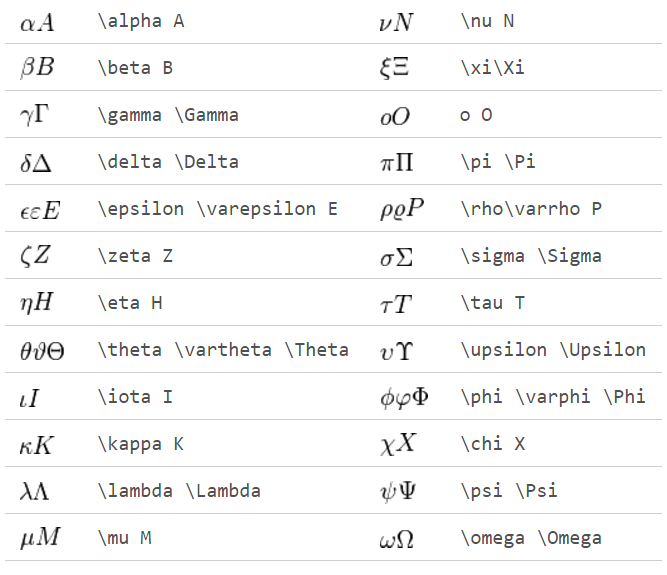
\includegraphics[width=0.8\textwidth]{Greek_letters}
\caption[Greek letters in \LaTeX]{List of Greek math letters in \LaTeX. Notice that italic uppercase letters are Latin italics; Greek uppercase letters are upright; if you want them inclined as the other lowercase Greek letters, and the Latin counterparts, you have to use the class command \texttt{\string\DeclareSlantedCapitalGreekLetters}.}
\label{fig:Greek}
\end{figure}


%\begin{landscape}

\paragraph{Subfigures}
A multiple figure example\footnote{This figure might have been typeset in landscape form by means of the \texttt{landscape} environment provided by the \texttt{lscape} package.} 
is presented here. Here you can refer any subfigure for example  arrows (see Fig.~\ref{fig:Arrows}) and binary operation symbols in (Fig.~\ref{fig:Miscsymb}) or you can cite the whole figure as Fig.~\ref{fig:Mathsymb}.

The \texttt{\char92textwidth} used in parametrising the various subfigures becomes the actual width of each subfigure material included with \texttt{\string\includegraphics}. This implies a non trivial amount of down scaling, and the included figures might become too thin, as it is evident in figure~\ref{fig:Mathsymb}. In most cases it is not wise to squeeze more than two figures in a row. In any case one or more spaces between two adjacent subfigures get such objects more distant from one another; a blank line between two adjacent subfigures behave as the start of a new paragraph even within the `figure' environment.


\begin{figure}[!hb]
  \centering
  \begin{subfigure}[b]{0.45\textwidth}
    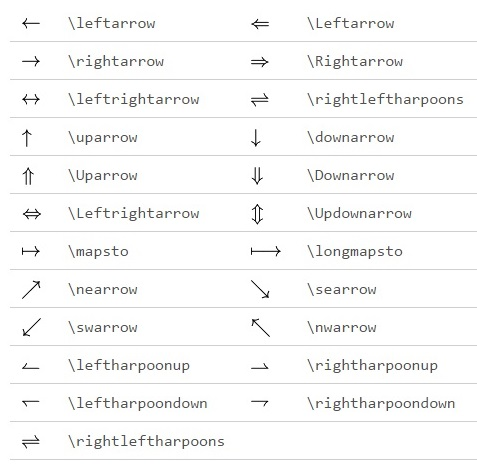
\includegraphics[width=\textwidth]{Arrows}
    \caption{Arrows}
    \label{fig:Arrows}   
  \end{subfigure}%
  \begin{subfigure}[b]{0.45\textwidth}
    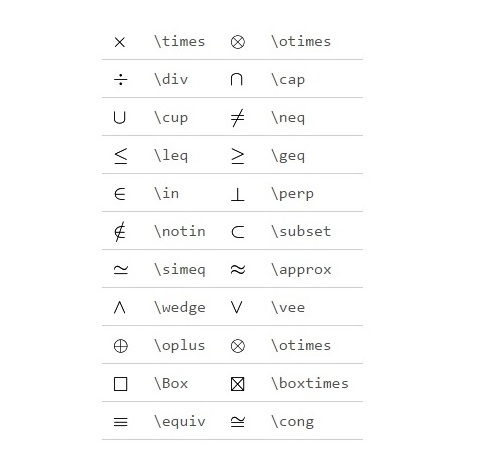
\includegraphics[width=\textwidth]{Binary_operations}
    \caption{Binary operator symbols}
    \label{fig:Binarysymb}
  \end{subfigure}%
  
  \begin{subfigure}[b]{0.45\textwidth}
    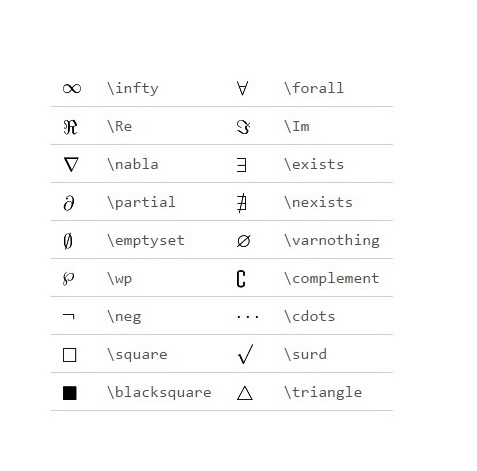
\includegraphics[width=\textwidth]{Miscellaneous_symbols}
    \caption{Miscellaneous symbols}
    \label{fig:Miscsymb}
  \end{subfigure}
  \caption{Useful math symbols in \LaTeX}
  \label{fig:Mathsymb}

\end{figure}

Another example with figures of a graphic type is shown in figure~\ref{fig:threedrawings}. As it can be seen the three subfigures have been strongly reduced, but their quality is not diminished as it was with the example in figure~\ref{fig:Mathsymb}.

\begin{figure}[!htb]
\centering
\begin{subfigure}[b]{0.3\textwidth}

\includegraphics[width=\textwidth]{minion}
\caption{Two minions}
\label{sfig:A}
\end{subfigure}
\hfill
\begin{subfigure}[b]{0.3\textwidth}

\includegraphics[width=\textwidth]{TomandJerry}
\caption{Tom and Jerry}
\label{sfig:B}
\end{subfigure}
\hfill
\begin{subfigure}[b]{0.3\textwidth}
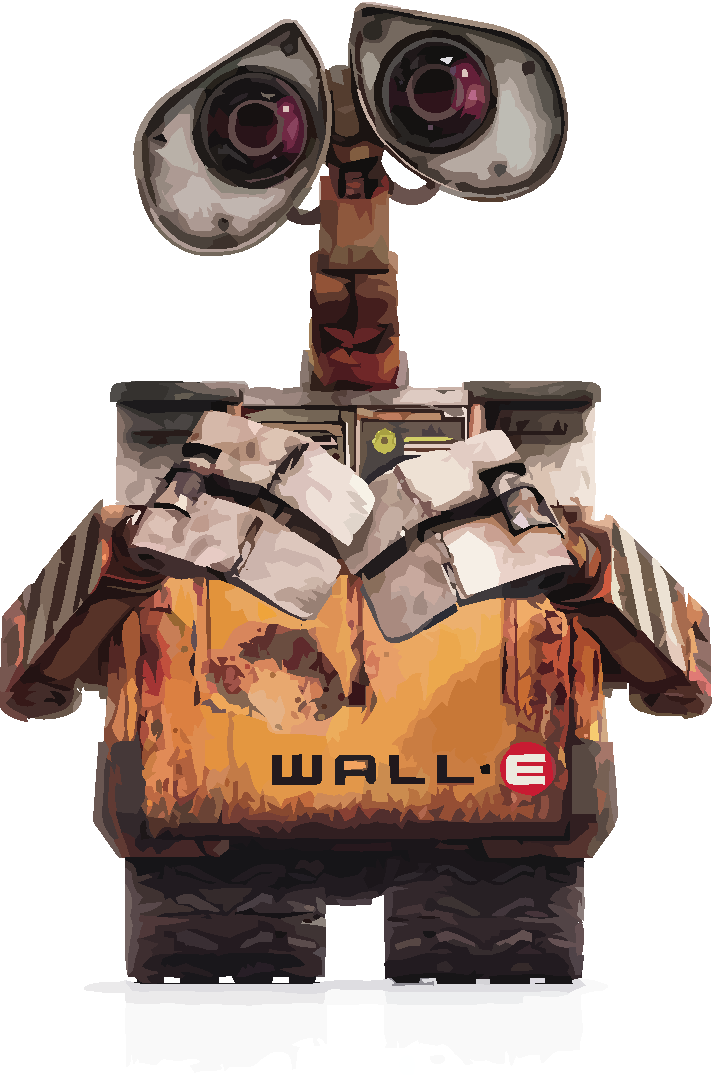
\includegraphics[width=\textwidth]{WallE}
\caption{Wall-E}
\label{sfig:C}
\end{subfigure}
\caption{Three drawings}
\label{fig:threedrawings}
\end{figure}

%\end{landscape}

%********************************** 
% Senventh Section  
\section{Tables}
%**********************************

The layout of a table has been established over centuries of experience and should only be altered in extraordinary circumstances \cite{fear2005publication}. 

When formatting a table, remember two simple guidelines at all times.
%
\begin{enumerate}
	\item Never, ever use vertical rules (lines).
	\item Never use double rules.
\end{enumerate}

These guidelines may seem extreme but I have never found a good argument in favour of breaking them. For example, if you feel that the information in the left half of a table is so different from that on the right that it needs to be separated by a vertical line, then you should use two tables instead. There are amateur typographers who don't follow the second guideline.

There are three further guidelines worth mentioning here as they
are generally not known outside the circle of professional
typesetters and subeditors:
\begin{enumerate}\setcounter{enumi}{2}
	\item Put the units of measure in the column heading (not in the body of
	the table).
	\item Always precede a decimal point by a digit; thus 0.1 
	{\em not} just .1.
	\item Do not use `ditto' signs or any other such convention to
	repeat a previous value. In many circumstances a blank
	will serve just as well. If it won't, then repeat the value.
	\item Numerical columns look better if the units are vertically aligned; 
	for this purpose package \texttt{siunitx} provides the special column \texttt{S} (that can be customised) in order to obtain this result. Nevertheless, if within the \texttt{table} environment the active character \texttt{\string~} is (locally) redefined so as to insert an invisible zero digit, it is not difficult to produce such vertical alignment by simply inserting this tilde sign before and/or after each fractional number. This method was used to typeset table~\ref{table:good_table}.
\end{enumerate}
A frequently mistake is to use `\texttt{\string\begin\{center\}...\string\end\{center\}}' inside a figure or table environment. This \texttt{center} environment can cause additional vertical space. If you want to avoid that, just use \texttt{\string\centering}.

\begin{table}
	\caption{A badly formatted table}
	\centering
	\label{table:bad_table}
	\begin{tabular}{|l|c|c|c|c|}
		\hline 
		& \multicolumn{2}{c}{Species I} & \multicolumn{2}{c|}{Species II} \\ 
		\hline
		Dental measurement  & mean & SD  & mean & SD  \\ \hline 
		\hline
		I1MD & 6.23 & 0.91 & 5.2  & 0.7  \\
		\hline 
		I1LL & 7.48 & 0.56 & 8.7  & 0.71 \\
		\hline 
		I2MD & 3.99 & 0.63 & 4.22 & 0.54 \\
		\hline 
		I2LL & 6.81 & 0.02 & 6.66 & 0.01 \\
		\hline 
		CMD & 13.47 & 0.09 & 10.55 & 0.05 \\
		\hline 
		CBL & 11.88 & 0.05 & 13.11 & 0.04\\ 
		\hline 
	\end{tabular}
\end{table}

\begin{table}
	\caption{A nice looking table}
	\centering
	\label{table:nice_table}
	\begin{tabular}{l c c c c}
		\hline 
		\multirow{2}{*}{Dental measurement} & \multicolumn{2}{c}{Species I} & \multicolumn{2}{c}{Species II} \\ 
		\cline{2-5}
		& mean & SD  & mean & SD  \\ 
		\hline
		I1MD & 6.23 & 0.91 & 5.2  & 0.7  \\
		
		I1LL & 7.48 & 0.56 & 8.7  & 0.71 \\
		
		I2MD & 3.99 & 0.63 & 4.22 & 0.54 \\
		
		I2LL & 6.81 & 0.02 & 6.66 & 0.01 \\
		
		CMD & 13.47 & 0.09 & 10.55 & 0.05 \\
		
		CBL & 11.88 & 0.05 & 13.11 & 0.04\\ 
		\hline 
	\end{tabular}
\end{table}


\begin{table}
	\caption{An even better looking table using \texttt{booktabs}}
	\centering
	\label{table:good_table}
	\def~{\phantom{0}}%
	\begin{tabular}{l c c c c}
		\toprule
% with booktabs it's better to lower the column heading by means
% of \raisebox with a negative "raise", instead of \multirow.
		\raisebox{-1.7ex}[0pt][0pt]{Dental measurement} & \multicolumn{2}{c}{Species I} & \multicolumn{2}{c}{Species II} \\ 
		\cmidrule{2-5}
		& mean & SD  & mean & SD  \\ 
		\midrule
		I1MD & ~6.23 & 0.91 & ~5.2~ & 0.7~ \\
		
		I1LL & ~7.48 & 0.56 & ~8.7~ & 0.71 \\
		
		I2MD & ~3.99 & 0.63 & ~4.22 & 0.54 \\
		
		I2LL & ~6.81 & 0.02 & ~6.66 & 0.01 \\
		
		CMD  & 13.47 & 0.09 & 10.55 & 0.05 \\
		
		CBL  & 11.88 & 0.05 & 13.11 & 0.04 \\ 
		\bottomrule
	\end{tabular}
\end{table}


%*********************************************** 
% Eighth Section  
\section{How to produce an archivable PDF file}
%***********************************************

To produce an archivable PDF file that satisfies regulation ISO 19005:2005-1b (PDF/A-1b) or 19005:2005-2b (PDF/A-2b) you should use pdfLaTeX or LuaLaTeX. With XeLeTeX it would also be possible, but it is necessary to execute by hand some postprocessing. So it is better to abide from XeLaTeX. 

With this TOPtesi bundle it should be possible to produce PDF/A compliant files, but 8-bit encoded fonts may give rise to problems; this bundle “repairs” some of these problems, but it is not guaranteed that repairs all problems arising from such fonts. Conformance to level PDF/A-2b is easier to be achieved if the thesis is typeset with LuaLaTeX.

The best solution is to typeset the Thesis with LuaLaTeX with the attention of not using any 8-bit encoded fonts, unless only (7-bit encoded)  \textsc{ascii} characters are used. This holds true also for imported figures that contain legends.

Imported figures should be preferred in vector formats; raster format is a second choice; the PNG raster format is to be preferred to the JPG one  when line drawings are imported, paying attention  that the file does not contain any transparency (for conformance level PDF/A-1b).

Metadata have to be added to the file; the best way to do it is to mimic what has been done in the source file of this document; that is to include the metadata in the form of a file generated by means of the \texttt{pdfxmetadata} environment. The data must be written in a form similar to the one used in this example file, but it is advisable to read the documentation of the \texttt{pdfx} package, to examine the fine details that are required.

Eventually the \texttt{pdfx} package needs to be loaded as the very first package after the \verb|\documentclass| statement, but after metadata have been spcified.

This very file has the initial part of the main file that looks as such:
{\small
\begin{verbatim}
%%%%%%% If and only if you want to produce an archivable
%%%%%%% document according to the ISO regulation
%%%%%%% 19005:2005-1b or -2b add the following code 
%%%%%%% at the beginning of your preamble.

\documentclass[12pt,twoside,scudo]{toptesi}
 
\begin{pdfxmetadata}{\jobname.xmpdata}
\Author{Mario Rossi}
\Title{Writing Your Ph.D. Thesis with LaTeX}
\Subject{Doctoral dissertations in the SCUDO doctoral school}
\Keywords{PDF\sep
          PDF/A\sep
          ISO 19005\sep
          LaTeX\sep
          PhD Thesis\sep
          Engineering\sep
          SCUDO}
\Publisher{Politecnico di Torino}
\end{pdfxmetadata}

\usepackage[a-2b]{pdfx}% or [a-1b]

%%%%
\end{verbatim}
}

The other necessary metadata are provided by the \texttt{pdfx} package. By typesetting the thesis with LuaLaTeX the chance of getting the PDF file already compliant at the first run is very high. But you cannot be sure unless you verify such compliance by means of one of these two methods.
\begin{enumerate}
\item
Download from the internet the VeraPDF software (the stable version is being available since 2017). Follow the simple instructions for creating on your computer the GUI variant of the program; this GUI is self explanatory for the actions to do for the verifications of your file. 
\item You have access to version XI or higher of the commercial Adobe Acrobat Pro software; open your file with this program, and verify its PDF/A compliance with Acrobat's module \texttt{Preflight}; its graphical interface is self explanatory.
\end{enumerate}
In each case, if the thesis PDF file is compliant print the report. If it is not compliant try to analyse the diagnostic messages, and correct what  turned to be wrong in your file.

This document has been typeset with LuaLaTeX and resulted compliant the very first time it was analysed. Well, this is a half truth; images in figure~\ref{fig:threedrawings} were not conformant because their color profiles, nominally RGB ones, were not actually so, therefore they caused the overall document to be a PDF/A non conformant one; their EPS sources were fetched and distilled again into PDF format so that every problem vanished.









	% Print bibliography and add to the TOC
	\nocite{*} % Include all bibliographic references in the document
	\printbibliography[heading=bibintoc]
	
\end{document}

